\chapter{Обработка информации с прибора} \label{chapt3}

Отладка программного обеспечения и проверка обработки сигналов от детекторов на этапе  конструкторских работ производилась подключением канала RS232 к последовательному (COM) порту персонального компьютера. Программное обеспечение контроллера формирует отладочные посылки и массивы тестовых данных и отправляет по интерфейсу USART, реализованному на всех использовавшихся контроллерах. Такой способ передачи тестовых данных выбран как максимально приближенный к условиям реального функционирования прибора. 

Отладка программного обеспечения и проверка обработки сигналов от детекторов на этапе  конструкторских работ производилась подключением канала RS232 к последовательному (COM) порту персонального компьютера. Программное обеспечение контроллера формирует отладочные посылки и массивы тестовых данных и отправляет по интерфейсу USART, реализованному на всех использовавшихся контроллерах. Такой способ передачи тестовых данных выбран как максимально приближенный к условиям реального функционирования прибора. 

Отработка работы прибора в комплексе научной аппаратуры позволяет использовать штатный способ передачи информации по каналу CAN, в таком случае критерием работы прибора является выдача от БИ содержательных блоков информации с меткой, соответствующей прибору ДЭПРОН. 

\section{Общая схема обработки и распределения потоков информации}\label{sec3.1}

Для обработки данных и отладки работы прибора ДЭПРОН были использованы специально разработанные программные средства. Поскольку отладка прибора ДЭПРОН производится подключением по каналу RS232 а при работе в штатном режиме передача данных ведется по каналу CAN, для взаимодействия с прибором были написаны две программы.

\subsection{Программа Depron Terminal}

Данная программа предназначена для отладки прибора во время лабораторных испытаний, проверки работоспособности прибора при приемо-сдаточных работах. Программа была написана в средстве разработки ПО Microsoft Visual Studio на языке C\#, c использованием фрэймворка .NET3.5. Пользовательский интерфейс программы построен на основе WinForms, поэтому отличается консервативностью и достаточно низкими аппаратными требованиями.

Программа позволяет:


\begin{itemize}
	\item 	Подключаться к прибору ДЭПРОН по каналу RS232 (с использованием COM порта)
	
	
	\item 	Принимать и отображать тестовые данные сформированные прибором ДЭПРОН
	
	
	\item 	Сохранять запись потока данных на жесткий диск ПК (в фоновом режиме и по запросу)
	
	
	\item 	Открывать сохраненные данные с носителя информации
	
	
	\item 	Посылать команды на прибор ДЭПРОН (в том числе с заданной периодичностью)
	
	
\end{itemize}
\begin{figure}
\centering
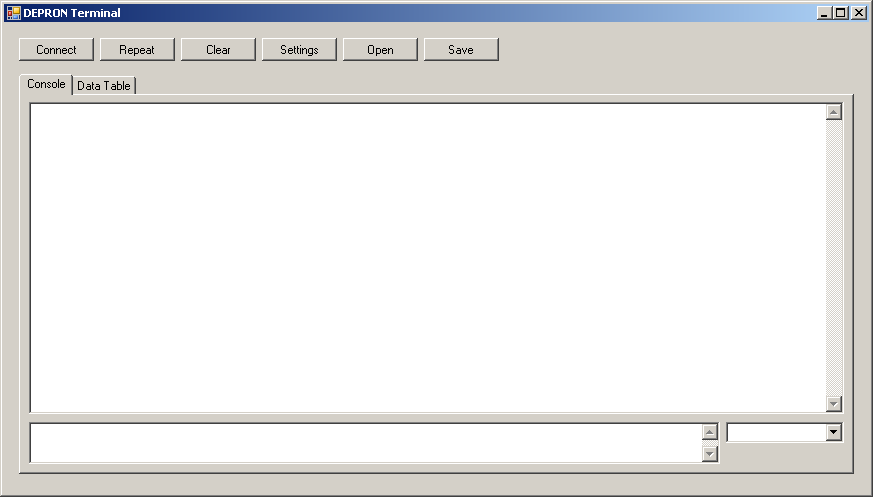
\includegraphics[width=0.7\linewidth]{images/depron_terminal}
\caption{Интерфейс программы \textbf{Depron Terminal}}
\label{fig:depron_terminal}
\end{figure}

Данная программа была использована как основа для разработки отладочной программы для дозиметрических блоков ДБ-8м. Основные принципы работы новой программы, названной \textbf{DB8m Terminal} были сохранены и она обеспечивает те же базовые функции. Дополнительно программа обеспечивает возможность накопления спектров энерговыделения по детекторам ДБ-8м и отображения их в графическом виде, в режиме реального времени. 
\begin{figure}
\centering
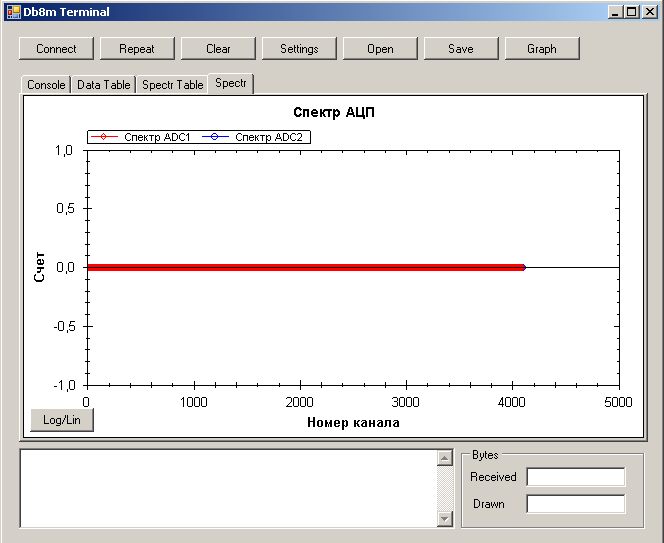
\includegraphics[width=0.7\linewidth]{images/db8m_terminal}
\caption{Интерфейс программы \textbf{DB8mTerminal}}
\label{fig:db8m_terminal}
\end{figure}

Графическое отображение спектров реализовано с использованием компонента ZedGraph. Введение такой возможности значительно ускорило калибровку и градуировку прибора на источниках радиационного излучения, так что может быть рекомендовано для программ аналогичной направленности.

\subsection{Программа DepronExplorerView}

Данная программа предназначена для просмотра и обработки данных прибора полученных во время комплексных испытаний или во время штатной работы прибора. Аналогично Depron Terminal, данная программа была написана в средстве разработки ПО Microsoft Visual Studio на языке c\# c использованием фрэймворка .NET3.5. Пользовательский интерфейс программы построен на основе WPF.


На момент комплексных испытаний прибора ДЭПРОН программа DepronExplorerView позволяет отображать все типы бинарных данных, полученных от прибора ДЭПРОН, в таблично-текстовой форме и сохранять полученные данные в текстовые файлы. Для удобства использования интерфейс программы выполнен в стиле файлового менеджера. 

Подготовленная программа активно использовлалась при всех испытаниях прибора ДЭПРОН в комплексе аппаратуры спутника, а также будет использоваться при предполетных проверках на космодроме Восточный.

\begin{figure}
\centering
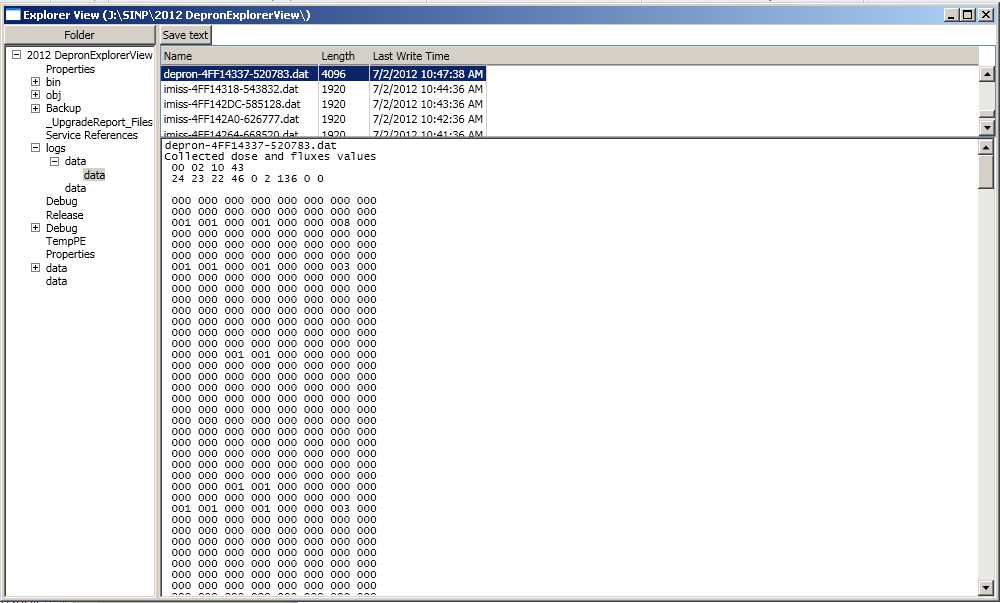
\includegraphics[width=0.8\linewidth]{images/depron_explorer}
\caption{Интерфейс программы \textbf{DepronExplorerView}}
\label{fig:depron_explorer}
\end{figure}


\subsection{Структура массивов (базы данных) результатов измерений}

Результаты измерений прибора ДЭПРОН формируется в массивы информации размером 512 байт.


Каждое сообщение состоит из следующих полей:

\begin{itemize}
	\item  начало сообщения;

	\item  категория;

	\item  длина сообщения;

	\item  данные.
\end{itemize}


Поле {``}начало сообщения'' содержит 2 байта:
\begin{itemize}
	\item байт DLE -- 11110000;
	\item байт STX -- 11111111.
\end{itemize}


На момент написания в программе ДЭПРОН используются нестандартные значения для байт DLE и STX, поэтому во избежание путаницы в дальнейших версия ПО ДЭПРОН будут использоваться общепринятые значения этих байт.


Поле ``категория'' состоит из одного байта (CAT). При обмене с БИ используются варианты сообщений: A, S, H, N. Коды сообщений соответствуют таблице ASCII: A - 01000001, S - 01010011, H - 01001000, N -- 01001110.

Поле ``длина сообщения'' содержит 1 байт (LEN) по умолчанию передается ``\ensuremath{\backslash 0}'', что означает общую длину посылки 512 байт.


В ином случае значение длины равно общему числу байт сообщения, исключая поле ``начало сообщения''.


Поле ``данные'' (RECORD) содержит данные в соответствии с описанием передаваемых сообщений и их спецификацией.



Общая структура сообщений выглядит следующим образом:

\begin{tabular}{|p{4.5cm}|c|c|p{2.5cm}|}
	\hline
	Начало сообщения (DLE,STX) & Категория(CAT) & Длина(LEN)  & Данные (RECORD) \\ \hline
	Метка 1                    & \multicolumn{2}{c|}{Метка 2} &  \\ \hline
	2 байта                    & \multicolumn{2}{c|}{2 байта} & {508 байт  }    \\ \hline
\end{tabular}

 
\subsection{Содержание блоков данных ДЭПРОН}

Прибор ДЭПРОН в процессе штатной работы формирует несколько типов массивов информации, которые соответствуют различным типам измерений:


\begin{itemize}
	\item 	дозиметрические измерения потока ионизирующих излучений;
	
	
	\item 	измерения спектров потока ионизирующих излучений;
	
	
	\item 	запись данных высокоэнергетичных событий в детекторах;
	
	
	\item 	измерение временного характера кратковременных нейтронных явлений;
	
	
\end{itemize}
Также прибор ДЭПРОН формирует ответ на пришедшую команду от БИ.





Типы массивов данных прибора ДЭПРОН:


\begin{itemize}
	\item 	блок данных ДЭПРОН  A  		Collected dose and fluxes values
	
	
	\item 	блок данных ДЭПРОН  S 		Energy deposition spectra
	
	
	\item 	блок данных ДЭПРОН  H  		High Amplitude Data
	
	
	\item 	блок данных ДЭПРОН  N		Neutron burst data
	
	
	\item 	блок данных ДЭПРОН  Т		квитанция на полученную команду
	

\end{itemize}

\subsection{Периодичность выдачи массивов данных}




\textbf{{\large Блок}}\textbf{{\large  }}\textbf{{\large данныхСодержаниеПериодичность}}{\small АВеличины поглощенной дозы и потоков частиц1 мин.}{\small S}{\small Спектр энерговыделения5 мин.}{\small H}{\small Данные о высокоэнергетичных событияхПо мере накопления данных}{\small N}{\small Данные по нейтронным вспышкамПо мере накопления данных, но не более 10 массивов в минуту}{\small T}{\small Квитанция на полученную командуПо мере поступления команд квитанция на полученную команду}{\small T[DEBUG]}{\small Данные по времени выполнения блоков программыПо мере заполнения буфера отправки сообщений прибора}


